% These are examples of Feynman Diagrams using TikZ
% Author: Flip Tanedo, 2010. pt267@cornell.edu

\documentclass[12pt]{article}	% Why do I use such a boring document clas?

% THE USUAL PACKAGES
\usepackage{amsmath,amssymb,amsfonts}	% DON'T use cite, screws with bibtex + hyperref
\usepackage{color}
\usepackage{amsmath}
\usepackage{amsfonts}
\usepackage{amssymb}
\usepackage{graphicx}
\usepackage{slashed}            % for slashed characters in math mode
\usepackage{bbm}                % for \mathbbm{1} (unit matrix)
\usepackage{xspace}				% For spacing after commands

\setcounter{MaxMatrixCols}{30}
\numberwithin{equation}{section} \setlength{\textwidth}{17.5cm}
\setlength{\textheight}{22.5cm} \setlength{\oddsidemargin}{-0.5cm}
\setlength{\evensidemargin}{1cm} \setlength{\headheight}{0cm}
\setlength{\headsep}{0cm} \setlength{\topmargin}{0cm}
\setlength{\footskip}{1.5cm} \baselineskip 0.6cm


% TIKZ - for drawing Feynman diagrams
% ... use with pdflatex

\usepackage{tikz}
\usetikzlibrary{arrows,shapes}
\usetikzlibrary{trees}
\usetikzlibrary{matrix,arrows} 				% For commutative diagram
											% http://www.felixl.de/commu.pdf
\usetikzlibrary{positioning}				% For "above of=" commands
\usetikzlibrary{calc,through}				% For coordinates
\usetikzlibrary{decorations.pathreplacing}  % For curly braces
% http://www.math.ucla.edu/~getreuer/tikz.html
\usepackage{pgffor}							% For repeating patterns

\usetikzlibrary{decorations.pathmorphing}	% For Feynman Diagrams
\usetikzlibrary{decorations.markings}
\tikzset{
	% >=stealth', %%  Uncomment for more conventional arrows
    vector/.style={decorate, decoration={snake}, draw},
	provector/.style={decorate, decoration={snake,amplitude=2.5pt}, draw},
	antivector/.style={decorate, decoration={snake,amplitude=-2.5pt}, draw},
    fermion/.style={draw=black, postaction={decorate},
        decoration={markings,mark=at position .55 with {\arrow[draw=black]{>}}}},
    fermionbar/.style={draw=black, postaction={decorate},
        decoration={markings,mark=at position .55 with {\arrow[draw=black]{<}}}},
    fermionnoarrow/.style={draw=black},
    gluon/.style={decorate, draw=black,
        decoration={coil,amplitude=4pt, segment length=5pt}},
    scalar/.style={dashed,draw=black, postaction={decorate},
        decoration={markings,mark=at position .55 with {\arrow[draw=black]{>}}}},
    scalarbar/.style={dashed,draw=black, postaction={decorate},
        decoration={markings,mark=at position .55 with {\arrow[draw=black]{<}}}},
    scalarnoarrow/.style={dashed,draw=black},
    electron/.style={draw=black, postaction={decorate},
        decoration={markings,mark=at position .55 with {\arrow[draw=black]{>}}}},
	bigvector/.style={decorate, decoration={snake,amplitude=4pt}, draw},
}

% TIKZ - for block diagrams, 
% from http://www.texample.net/tikz/examples/control-system-principles/
% \usetikzlibrary{shapes,arrows}
\tikzstyle{block} = [draw, rectangle, 
    minimum height=3em, minimum width=6em]


\usepackage{hyperref}			% Has to be at the end.



\begin{document}
\begin{titlepage}
\begin{flushright}
\end{flushright}

\begin{center}
{\huge\bf Feynman Diagrams}\\
{\Large \bf via TikZ}

\medskip
\bigskip\color{black}\vspace{0.6cm}
{
{\large\bf 
Flip Tanedo}
%% E.g.:
% {\large\bf Brando Bellazzini$^{a,b}$, Csaba Cs\'aki$^a$,\\[3mm] Antonio Delgado$^c$, and Andreas Weiler$^{a,d}$}
}
\\[7mm]
{\it Institute for High Energy Phenomenology,\\ Newman Laboratory of Elementary Particle Physics,\\
Cornell University, Ithaca, NY 14853, USA}
%% E.g. for multiple:
% {\it $^a$ Institute for High Energy Phenomenology,\\ Newman Laboratory of Elementary Particle Physics,\\
% Cornell University, Ithaca, NY 14853, USA} \\
% \vspace*{0.3cm}
% {\it $^b$ INFN, Sezione di Pisa,  Largo Pontecorvo 3, 56127, Pisa,
% Italy}
% \\
% \vspace*{0.3cm}
% {\it $^c$ Department of Physics, University of Notre Dame, Indiana 46556, USA} \\
% \vspace*{0.3cm}
% {\it $^d$ CERN Theory Division, CH-1211 Geneva 23, Switzerland}
\\
\vspace*{0.3cm}
{\it E-mail: \rm{
 \href{mailto:pt267@cornell.edu}{pt267@cornell.edu}}}
\bigskip

{\large \textbf{This version:} \today}

\bigskip\bigskip

{
\centerline{\large\bf Abstract}
\begin{quote}

These are sample Feynman diagrams.

\end{quote}}



\end{center}
\bigskip\bigskip
\setcounter{tocdepth}{2}
\tableofcontents
\end{titlepage}















\section{QED}


\vspace{2em}

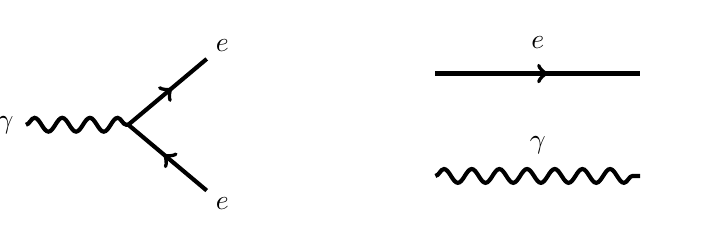
\begin{tikzpicture}[line width=1.5 pt, scale=1.3]
	\draw[fermion] (-40:1)--(0,0);
	\draw[fermionbar] (40:1)--(0,0);
	\draw[vector] (180:1)--(0,0);
	\node at (-40:1.2) {$e$};
	\node at (40:1.2) {$e$};
	\node at (180:1.2) {$\gamma$};
	\draw[fermion] (3,.5)--(5,.5);
	\draw[vector] (3,-.5)--(5,-.5);
	\node at (4, .8) {$e$};
	\node at (4, -.2) {$\gamma$};
 \end{tikzpicture}

\vspace{2em}
% 
% \begin{tikzpicture}[line width=1.5 pt, scale=1.3]
% \begin{scope}[shift={(0,.75)}]
% 	\draw[fermion](0,-2) -- (1,-1.75);
% 	\draw[fermion](1,-1.75) -- (2,- 1.5);
% 	\draw[fermion](2,-1.5) -- (3,-1.25);
% 	\draw[fermion](3,-1.25) -- (4,-1);
% 	\draw[vector](1,-1.75) -- (2,- 2.2);
% 	% \draw[vector](2,-1.5) -- (3,-1.95);
% 	\draw[vector](3,-1.25) -- (4,-1.7);
% \end{scope}
% \begin{scope}[shift={(0,-.75)}]
% 	\draw[fermionbar](0,2) -- (1,1.75);
% 	\draw[fermionbar](1,1.75) -- (2,1.5);
% 	\draw[fermionbar](2,1.5) -- (3,1.25);
% 	\draw[fermionbar](3,1.25) -- (4,1);
% 	\draw[vector](1,1.75) -- (2,2.2);
% 	% \draw[vector](2,1.5) -- (3,1.95);
% 	\draw[vector](3,1.25) -- (4,1.7);
% \end{scope}
% 	\draw[vector](2,-.75) -- (2,.75);
% \end{tikzpicture}
% 
% \vspace{2em}


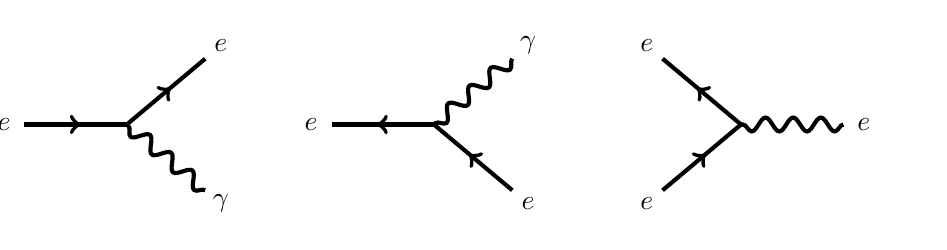
\begin{tikzpicture}[line width=1.5 pt, scale=1.3]
	\draw[vector] (-40:1)--(0,0);
	\draw[fermionbar] (40:1)--(0,0);
	\draw[fermion] (180:1)--(0,0);
	\node at (-40:1.2) {$\gamma$};
	\node at (40:1.2) {$e$};
	\node at (180:1.2) {$e$};	
\begin{scope}[shift={(3,0)}]
	\draw[fermion] (-40:1)--(0,0);
	\draw[vector] (40:1)--(0,0);
	\draw[fermionbar] (180:1)--(0,0);
	\node at (-40:1.2) {$e$};
	\node at (40:1.2) {$\gamma$};
	\node at (180:1.2) {$e$};	
\end{scope}
\begin{scope}[shift={(6,0)}]
			\draw[fermion] (-140:1)--(0,0);
			\draw[fermionbar] (140:1)--(0,0);
			\draw[vector] (0:1)--(0,0);
			\node at (-140:1.2) {$e$};
			\node at (140:1.2) {$e$};
			\node at (0:1.2) {$e$};	
\end{scope}
\end{tikzpicture}

\vspace{1em}
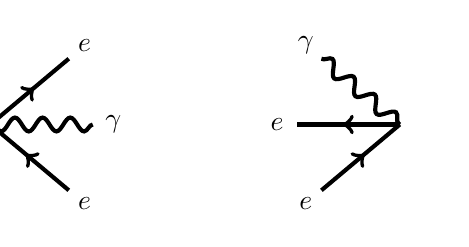
\begin{tikzpicture}[line width=1.5 pt, scale=1.3]
	\draw[fermion] (-40:1)--(0,0);
	\draw[fermionbar] (40:1)--(0,0);
	\draw[vector] (0:1)--(0,0);
	\node at (-40:1.2) {$e$};
	\node at (40:1.2) {$e$};
	\node at (0:1.2) {$\gamma$};	
\begin{scope}[shift={(4,0)}]
	\draw[fermion] (-140:1)--(0,0);
	\draw[vector] (140:1)--(0,0);
	\draw[fermionbar] (180:1)--(0,0);
	\node at (-140:1.2) {$e$};
	\node at (140:1.2) {$\gamma$};
	\node at (180:1.2) {$e$};	
\end{scope}
\end{tikzpicture}


\vspace{1em}
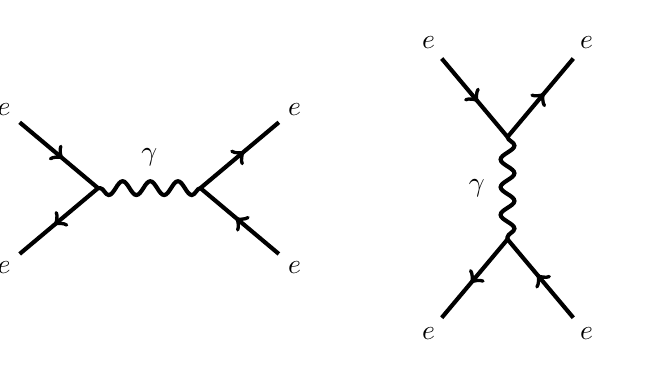
\begin{tikzpicture}[line width=1.5 pt, scale=1.3]
	\draw[fermionbar] (-140:1)--(0,0);
	\draw[fermion] (140:1)--(0,0);
	\draw[vector] (0:1)--(0,0);
	\node at (-140:1.2) {$e$};
	\node at (140:1.2) {$e$};
	\node at (.5,.3) {$\gamma$};	
\begin{scope}[shift={(1,0)}]
	\draw[fermion] (-40:1)--(0,0);
	\draw[fermionbar] (40:1)--(0,0);
	\node at (-40:1.2) {$e$};
	\node at (40:1.2) {$e$};	
\end{scope}
\begin{scope}[shift={(4,-.5)}]
	\begin{scope}[rotate=90]
			\draw[fermion] (-140:1)--(0,0);
			\draw[fermionbar] (140:1)--(0,0);
			\draw[vector] (0:1)--(0,0);
			\node at (-140:1.2) {$e$};
			\node at (140:1.2) {$e$};
			\node at (.5,.3) {$\gamma$};	
		\begin{scope}[shift={(1,0)}]
			\draw[fermionbar] (-40:1)--(0,0);
			\draw[fermion] (40:1)--(0,0);
			\node at (-40:1.2) {$e$};
			\node at (40:1.2) {$e$};	
		\end{scope}
	\end{scope}
\end{scope}
\end{tikzpicture}

\vspace{2em}

\vspace{1em}
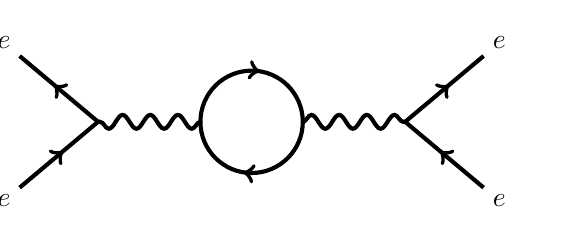
\begin{tikzpicture}[line width=1.5 pt, scale=1.3]
	\draw[fermion] (-140:1)--(0,0);
	\draw[fermionbar] (140:1)--(0,0);
	\draw[vector] (0:1)--(0,0);
	\node at (-140:1.2) {$e$};
	\node at (140:1.2) {$e$};
	% \node at (.5,.3) {$\gamma$};	
	\draw[fermion] (1,0) arc (180:0:.5);
	\draw[fermion] (2,0) arc (0:-180:.5);
	\draw[vector] (2,0) --(3,0);
	% \node at (2.5,.3) {$\gamma$};	
\begin{scope}[shift={(3,0)}]
	\draw[fermion] (-40:1)--(0,0);
	\draw[fermionbar] (40:1)--(0,0);
	\node at (-40:1.2) {$e$};
	\node at (40:1.2) {$e$};	
\end{scope}
\end{tikzpicture}

\vspace{1em}
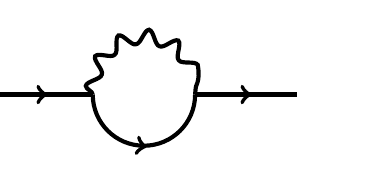
\begin{tikzpicture}[line width=1.5 pt, scale=1.3]
	\draw[fermionbar] (0:1)--(0,0);
	% \node at (-140:1.2) {$e$};
	% \node at (140:1.2) {$e$};
	% \node at (.5,.3) {$\gamma$};	
	\draw[vector] (1,0) arc (180:0:.5);
	\draw[fermionbar] (2,0) arc (0:-180:.5);
	\draw[fermion] (2,0) --(3,0);
	% \node at (2.5,.3) {$\gamma$};	
\end{tikzpicture}

\vspace{1em}
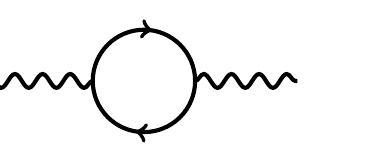
\begin{tikzpicture}[line width=1.5 pt, scale=1.3]
	\draw[vector] (0:1)--(0,0);
	\draw[fermion] (1,0) arc (180:0:.5);
	\draw[fermion] (2,0) arc (0:-180:.5);
	\draw[vector] (2,0) --(3,0);
\end{tikzpicture}


\vspace{1em}
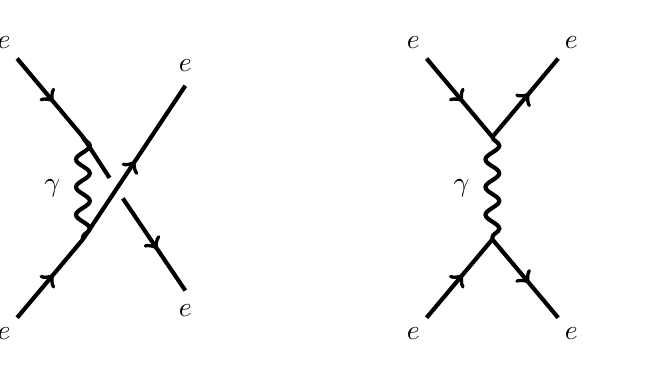
\begin{tikzpicture}[line width=1.5 pt, scale=1.3]
	\begin{scope}[rotate=90]
			\draw[fermionbar] (1.5,-1)--(0,0);
			\draw[fermion] (140:1)--(0,0);
			\draw[vector] (0:1)--(0,0);
			\node at (1.7,-1) {$e$};
			\node at (140:1.2) {$e$};
			\node at (.5,.3) {$\gamma$};	
		\begin{scope}[shift={(1,0)}]
			% \draw[fermionbar] (-1.5,-1)--(0,0);
			\draw[fermionnoarrow] (-.4,-.26)--(0,0);
			\draw[fermion] (-.6,-.39)--(-1.5,-1);
			\draw[fermion] (40:1)--(0,0); %top left
			\node at (-1.7,-1) {$e$};
			\node at (40:1.2) {$e$};	
		\end{scope}
	\end{scope}
\begin{scope}[shift={(4,0)}]
	\begin{scope}[rotate=90]
			\draw[fermionbar] (-140:1)--(0,0);
			\draw[fermion] (140:1)--(0,0);
			\draw[vector] (0:1)--(0,0);
			\node at (-140:1.2) {$e$};
			\node at (140:1.2) {$e$};
			\node at (.5,.3) {$\gamma$};	
		\begin{scope}[shift={(1,0)}]
			\draw[fermionbar] (-40:1)--(0,0);
			\draw[fermion] (40:1)--(0,0);
			\node at (-40:1.2) {$e$};
			\node at (40:1.2) {$e$};	
		\end{scope}
	\end{scope}
\end{scope}
\end{tikzpicture}


\section{QED+$\mu$}

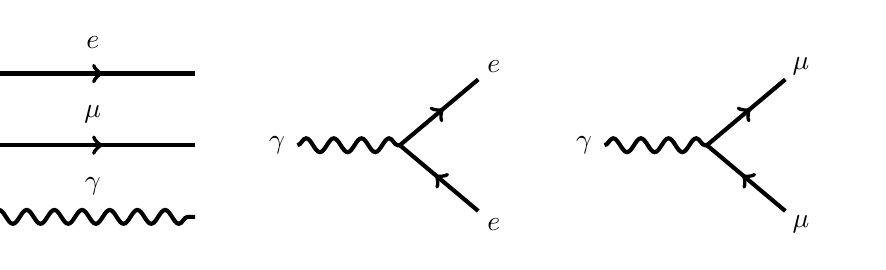
\begin{tikzpicture}[line width=1.5 pt, scale=1.3]
	\draw[fermion] (0,.7)--(2,.7);
	\draw[fermion] (0,.0)--(2,.0);
	\draw[vector] (0,-.7)--(2,-.7);
	\node at (1, 1) {$e$};
	\node at (1, 0.3) {$\mu$};
	\node at (1, -.4) {$\gamma$};
%
\begin{scope}[shift={(4,0)}]
	\draw[fermion] (-40:1)--(0,0);
	\draw[fermionbar] (40:1)--(0,0);
	\draw[vector] (180:1)--(0,0);
	\node at (-40:1.2) {$e$};
	\node at (40:1.2) {$e$};
	\node at (180:1.2) {$\gamma$};	
\end{scope}
\begin{scope}[shift={(7,0)}]
	\draw[fermion] (-40:1)--(0,0);
	\draw[fermionbar] (40:1)--(0,0);
	\draw[vector] (180:1)--(0,0);
	\node at (-40:1.2) {$\mu$};
	\node at (40:1.2) {$\mu$};
	\node at (180:1.2) {$\gamma$};	
\end{scope}
\end{tikzpicture}

Electrons to muons

\vspace{1em}
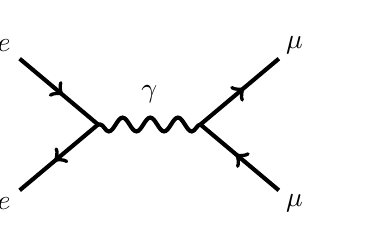
\begin{tikzpicture}[line width=1.5 pt, scale=1.3]
	\draw[fermionbar] (-140:1)--(0,0);
	\draw[fermion] (140:1)--(0,0);
	\draw[vector] (0:1)--(0,0);
	\node at (-140:1.2) {$e$};
	\node at (140:1.2) {$e$};
	\node at (.5,.3) {$\gamma$};	
\begin{scope}[shift={(1,0)}]
	\draw[fermion] (-40:1)--(0,0);
	\draw[fermionbar] (40:1)--(0,0);
	\node at (-40:1.2) {$\mu$};
	\node at (40:1.2) {$\mu$};	
\end{scope}
\end{tikzpicture}

\vspace{1em}

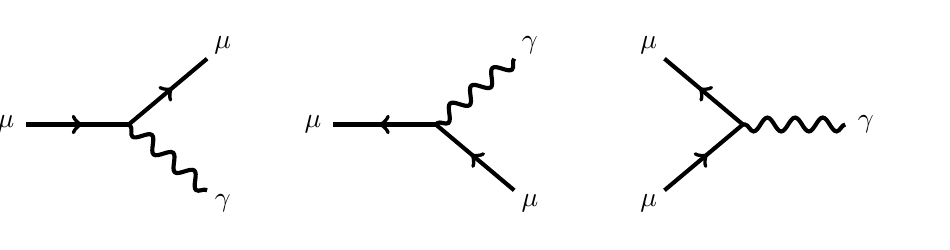
\begin{tikzpicture}[line width=1.5 pt, scale=1.3]
	\draw[vector] (-40:1)--(0,0);
	\draw[fermionbar] (40:1)--(0,0);
	\draw[fermion] (180:1)--(0,0);
	\node at (-40:1.2) {$\gamma$};
	\node at (40:1.2) {$\mu$};
	\node at (180:1.2) {$\mu$};	
\begin{scope}[shift={(3,0)}]
	\draw[fermion] (-40:1)--(0,0);
	\draw[vector] (40:1)--(0,0);
	\draw[fermionbar] (180:1)--(0,0);
	\node at (-40:1.2) {$\mu$};
	\node at (40:1.2) {$\gamma$};
	\node at (180:1.2) {$\mu$};	
\end{scope}
\begin{scope}[shift={(6,0)}]
			\draw[fermion] (-140:1)--(0,0);
			\draw[fermionbar] (140:1)--(0,0);
			\draw[vector] (0:1)--(0,0);
			\node at (-140:1.2) {$\mu$};
			\node at (140:1.2) {$\mu$};
			\node at (0:1.2) {$\gamma$};	
\end{scope}
\end{tikzpicture}

\vspace{1em}
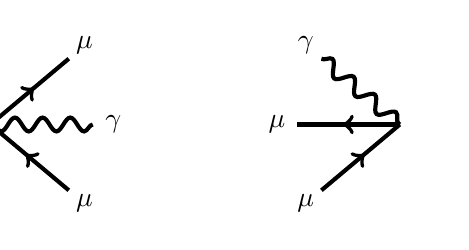
\begin{tikzpicture}[line width=1.5 pt, scale=1.3]
	\draw[fermion] (-40:1)--(0,0);
	\draw[fermionbar] (40:1)--(0,0);
	\draw[vector] (0:1)--(0,0);
	\node at (-40:1.2) {$\mu$};
	\node at (40:1.2) {$\mu$};
	\node at (0:1.2) {$\gamma$};	
\begin{scope}[shift={(4,0)}]
	\draw[fermion] (-140:1)--(0,0);
	\draw[vector] (140:1)--(0,0);
	\draw[fermionbar] (180:1)--(0,0);
	\node at (-140:1.2) {$\mu$};
	\node at (140:1.2) {$\gamma$};
	\node at (180:1.2) {$\mu$};	
\end{scope}
\end{tikzpicture}


\section{QED+$Z$+$\mu$}

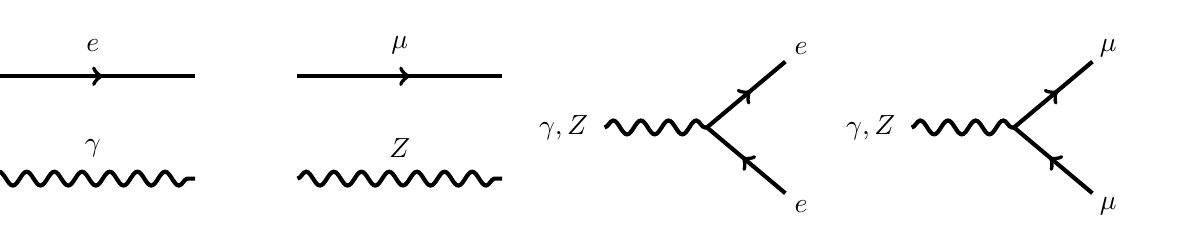
\begin{tikzpicture}[line width=1.5 pt, scale=1.3]
	\draw[fermion] (0,.5)--(2,.5);
	\draw[vector] (0,-.5)--(2,-.5);
	\node at (1, .8) {$e$};
	\node at (1, -.2) {$\gamma$};
%
\draw[fermion] (3,.5)--(5,.5);
\draw[vector] (3,-.5)--(5,-.5);
\node at (4, .8) {$\mu$};
\node at (4, -.2) {$Z$};
%
\begin{scope}[shift={(7,0)}]
	\draw[fermion] (-40:1)--(0,0);
	\draw[fermionbar] (40:1)--(0,0);
	\draw[vector] (180:1)--(0,0);
	\node at (-40:1.2) {$e$};
	\node at (40:1.2) {$e$};
	\node at (180:1.4) {$\gamma, Z$};	
\end{scope}
\begin{scope}[shift={(10,0)}]
	\draw[fermion] (-40:1)--(0,0);
	\draw[fermionbar] (40:1)--(0,0);
	\draw[vector] (180:1)--(0,0);
	\node at (-40:1.2) {$\mu$};
	\node at (40:1.2) {$\mu$};
	\node at (180:1.4) {$\gamma, Z$};	
\end{scope}\end{tikzpicture}

% \begin{scope}[shift={(220:1)}]
% 	\draw (125:.1) -- (-55:.1);
% 	\draw (55:.1) -- (-125:.1);			
% \end{scope}

\vspace{1cm}

Electrons to muons via $Z$

\vspace{1em}
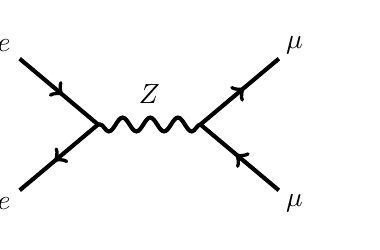
\begin{tikzpicture}[line width=1.5 pt, scale=1.3]
	\draw[fermionbar] (-140:1)--(0,0);
	\draw[fermion] (140:1)--(0,0);
	\draw[vector] (0:1)--(0,0);
	\node at (-140:1.2) {$e$};
	\node at (140:1.2) {$e$};
	\node at (.5,.3) {$Z$};	
\begin{scope}[shift={(1,0)}]
	\draw[fermion] (-40:1)--(0,0);
	\draw[fermionbar] (40:1)--(0,0);
	\node at (-40:1.2) {$\mu$};
	\node at (40:1.2) {$\mu$};	
\end{scope}
\end{tikzpicture}

\vspace{1em}
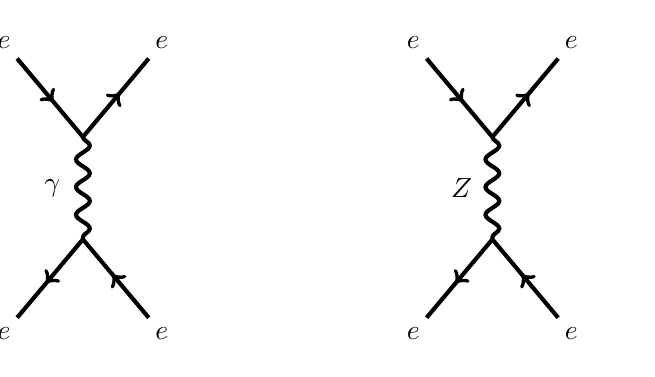
\begin{tikzpicture}[line width=1.5 pt, scale=1.3]
	\begin{scope}[rotate=90]
			\draw[fermion] (-140:1)--(0,0);
			\draw[fermionbar] (140:1)--(0,0);
			\draw[vector] (0:1)--(0,0);
			\node at (-140:1.2) {$e$};
			\node at (140:1.2) {$e$};
			\node at (.5,.3) {$\gamma$};	
		\begin{scope}[shift={(1,0)}]
			\draw[fermionbar] (-40:1)--(0,0);
			\draw[fermion] (40:1)--(0,0);
			\node at (-40:1.2) {$e$};
			\node at (40:1.2) {$e$};	
		\end{scope}
	\end{scope}
\begin{scope}[shift={(4,0)}]
	\begin{scope}[rotate=90]
			\draw[fermion] (-140:1)--(0,0);
			\draw[fermionbar] (140:1)--(0,0);
			\draw[vector] (0:1)--(0,0);
			\node at (-140:1.2) {$e$};
			\node at (140:1.2) {$e$};
			\node at (.5,.3) {$Z$};	
		\begin{scope}[shift={(1,0)}]
			\draw[fermionbar] (-40:1)--(0,0);
			\draw[fermion] (40:1)--(0,0);
			\node at (-40:1.2) {$e$};
			\node at (40:1.2) {$e$};	
		\end{scope}
	\end{scope}
\end{scope}

\end{tikzpicture}



\section{Blob diagrams}

% \begin{tikzpicture}[line width=1.5 pt, scale=2.5]
% 	\draw[fill=black] (0,0) circle (.3cm);
% 	\draw[fill=white] (0,0) circle (.29cm);
% 	\begin{scope}
%     	\clip (0,0) circle (.3cm);
%     	\foreach \x in {-.9,-.8,...,.3}
% 			\draw[line width=1 pt] (\x,-.3) -- (\x+.6,.3);
%   	\end{scope}
%  \end{tikzpicture}
% 
% Dark Matter:

% \begin{center}
	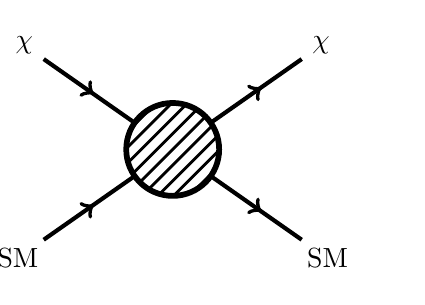
\begin{tikzpicture}[line width=1.5 pt, scale=2]
		\draw[fermion](145:1) -- (145:.3cm);
			\node at (145:1.15) {$\chi$};
		\draw[fermion](215:1) -- (215:.3cm);
			\node at (215:1.2) {SM};
		\draw[fermionbar](35:1) -- (35:.3cm);
			\node at (35:1.15) {$\chi$};
		\draw[fermionbar](-35:1) -- (-35:.3cm);
			\node at (-35:1.2) {SM};
		\draw[fill=black] (0,0) circle (.3cm);
		\draw[fill=white] (0,0) circle (.29cm);
		\begin{scope}
	    	\clip (0,0) circle (.3cm);
	    	\foreach \x in {-.9,-.8,...,.3}
				\draw[line width=1 pt] (\x,-.3) -- (\x+.6,.3);
	  	\end{scope}
	 \end{tikzpicture}	
% \end{center}



\section{Coleman Weinberg}

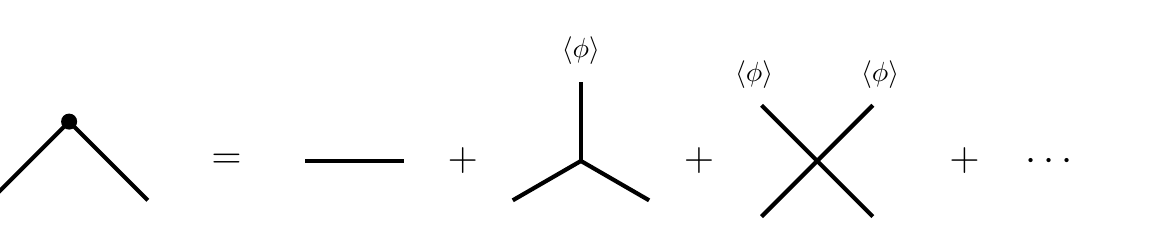
\begin{tikzpicture}[line width=1.5 pt]
	\draw (-1,-.5) -- (0,.5) -- (1,-.5);
	\draw[fill=black] (0,.5) circle (.075cm);
	\node at (2,0) {\Large=};
	\draw (3,0) -- (4.25,0);
	\node at (5,0) {\Large+};
	\draw (-30:1)+(6.5,0) -- (6.5,0);
	\draw (90:1)+(6.5,0) -- (6.5,0);
	\draw (210:1)+(6.5,0) -- (6.5,0);
	\node at (6.5,1.4) {$\langle \phi\rangle$};
	\node at (8,0) {\Large+};
	\draw (45:1)+(9.5,0) -- (9.5,0);
	\draw (135:1)+(9.5,0) -- (9.5,0);
	\draw (225:1)+(9.5,0) -- (9.5,0);
	\draw (315:1)+(9.5,0) -- (9.5,0);
	\node at (8.7,1.1) {$\langle \phi\rangle$};
	\node at (10.3,1.1) {$\langle \phi\rangle$};
	\node at (12,0) {\Large$+\hspace{.5cm}\cdots$};
 \end{tikzpicture}


\section{'t Hooft operator}


	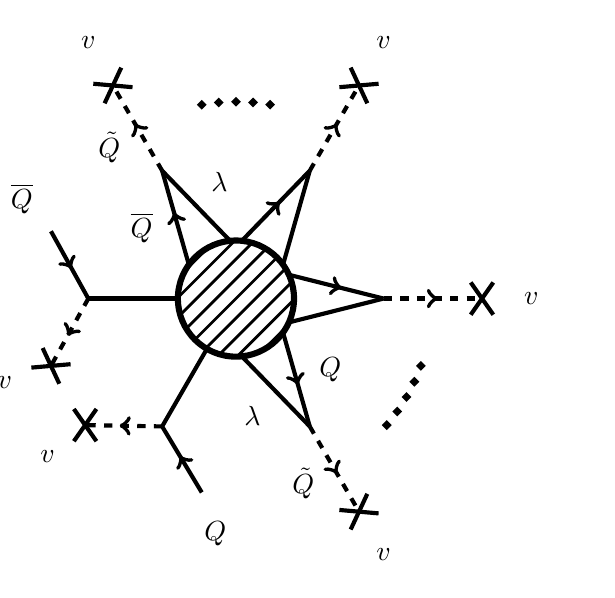
\begin{tikzpicture}[line width=1.5 pt, scale=2.5]
		\draw[fermionbar] (0:.75) -- (25:.29);
		\draw[fermionnoarrow] (0:.75) -- (-25:.29);
		\draw[scalar] (0:.75) -- (0:1.25);
		\begin{scope}[shift={(1.25,0)}]
			\draw (125:.1) -- (-55:.1);
			\draw (55:.1) -- (-125:.1);			
		\end{scope}
		\draw[fermionbar] (60:.75) -- (85:.29);
		\draw[fermionnoarrow] (60:.75) -- (35:.29);
		\draw[scalar] (60:.75) -- (60:1.25);
		\begin{scope}[shift={(60:1.25)}, rotate=60]
			\draw (125:.1) -- (-55:.1);
			\draw (55:.1) -- (-125:.1);			
		\end{scope}
		\draw[fermionbar] (120:.75) -- (145:.29);
		\draw[fermionnoarrow] (120:.75) -- (95:.29);
		\draw[scalar] (120:.75) -- (120:1.25);
		\begin{scope}[shift={(120:1.25)}, rotate=120]
			\draw (125:.1) -- (-55:.1);
			\draw (55:.1) -- (-125:.1);			
		\end{scope}
		\draw[fermionbar] (300:.75) -- (325:.29);
		\draw[fermionnoarrow] (300:.75) -- (275:.29);
		\draw[scalar] (300:.75) -- (300:1.25);
		\begin{scope}[shift={(300:1.25)}, rotate=300]
			\draw (125:.1) -- (-55:.1);
			\draw (55:.1) -- (-125:.1);			
		\end{scope}
		\draw[fill=black] (320:1) circle (.01);
		\draw[fill=black] (325:1) circle (.01);
		\draw[fill=black] (330:1) circle (.01);
		\draw[fill=black] (335:1) circle (.01);
		\draw[fill=black] (340:1) circle (.01);
		\draw[fill=black] (80:1) circle (.01);
		\draw[fill=black] (85:1) circle (.01);
		\draw[fill=black] (90:1) circle (.01);
		\draw[fill=black] (95:1) circle (.01);
		\draw[fill=black] (100:1) circle (.01);
		\draw[fill=black] (0,0) circle (.3cm);
		\draw[fill=white] (0,0) circle (.29cm);
		\begin{scope}
	    	\clip (0,0) circle (.3cm);
	    	\foreach \x in {-.9,-.8,...,.3}
				\draw[line width=1 pt] (\x,-.3) -- (\x+.6,.3);
	  	\end{scope}
		% \node at (0,0) {I};
		\node at (278:.6) {$\lambda$};
		\node at (323:.6) {$Q$};
		\node at (98:.6) {$\lambda$};
		\node at (143:.6) {$\overline Q$};
		\node at (290:1) {$\tilde Q$};
		\node at (130:1) {$\tilde Q$};
		\node at (300:1.5) {$v$};
		\node at (120:1.5) {$v$};
		\node at (60:1.5) {$v$};
		\node at (0:1.5) {$v$};
		\draw[fermionnoarrow] (180:.75) -- (180:.29);
		\draw[fermionnoarrow] (240:.75) -- (240:.29);
		\draw[fermion] (160:1) -- (180:.75);
		\draw[scalar] (180:.75) -- (200:1);
		\begin{scope}[shift={(200:1)}, rotate=60]
			\draw (125:.1) -- (-55:.1);
			\draw (55:.1) -- (-125:.1);			
		\end{scope}
		\draw[fermion] (260:1) -- (240:.75);
		\draw[scalar] (240:.75) -- (220:1);
		\begin{scope}[shift={(220:1)}]
			\draw (125:.1) -- (-55:.1);
			\draw (55:.1) -- (-125:.1);			
		\end{scope}
		\node at (200:1.25) {$v$};
		\node at (220:1.25) {$v$};
		\node at (265:1.2) {$Q$};
		\node at (155:1.2) {$\overline Q$};
	 \end{tikzpicture}
	
	\vspace{2em}
	
	
	
	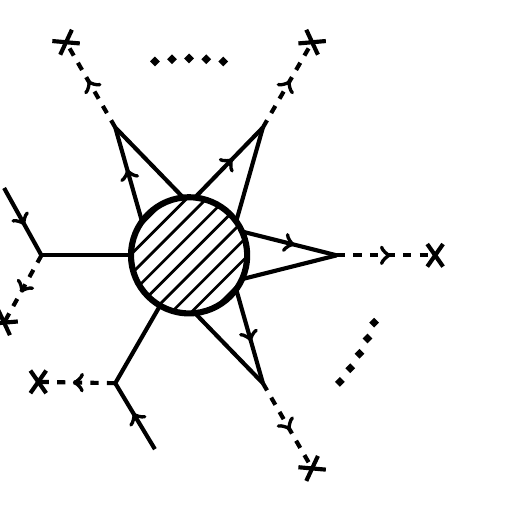
\begin{tikzpicture}[line width=1.5 pt, scale=2.5]
		\draw[fermionbar] (0:.75) -- (25:.29);
		\draw[fermionnoarrow] (0:.75) -- (-25:.29);
		\draw[scalar] (0:.75) -- (0:1.25);
		\begin{scope}[shift={(1.25,0)}]
			\draw (125:.07) -- (-55:.07);
			\draw (55:.07) -- (-125:.07);			
		\end{scope}
		\draw[fermionbar] (60:.75) -- (85:.29);
		\draw[fermionnoarrow] (60:.75) -- (35:.29);
		\draw[scalar] (60:.75) -- (60:1.25);
		\begin{scope}[shift={(60:1.25)}, rotate=60]
			\draw (125:.07) -- (-55:.07);
			\draw (55:.07) -- (-125:.07);
		\end{scope}
		\draw[fermionbar] (120:.75) -- (145:.29);
		\draw[fermionnoarrow] (120:.75) -- (95:.29);
		\draw[scalar] (120:.75) -- (120:1.25);
		\begin{scope}[shift={(120:1.25)}, rotate=120]
			\draw (125:.07) -- (-55:.07);
			\draw (55:.07) -- (-125:.07);
		\end{scope}
		\draw[fermionbar] (300:.75) -- (325:.29);
		\draw[fermionnoarrow] (300:.75) -- (275:.29);
		\draw[scalar] (300:.75) -- (300:1.25);
		\begin{scope}[shift={(300:1.25)}, rotate=300]
			\draw (125:.07) -- (-55:.07);
			\draw (55:.07) -- (-125:.07);
		\end{scope}
		\draw[fill=black] (320:1) circle (.01);
		\draw[fill=black] (325:1) circle (.01);
		\draw[fill=black] (330:1) circle (.01);
		\draw[fill=black] (335:1) circle (.01);
		\draw[fill=black] (340:1) circle (.01);
		\draw[fill=black] (80:1) circle (.01);
		\draw[fill=black] (85:1) circle (.01);
		\draw[fill=black] (90:1) circle (.01);
		\draw[fill=black] (95:1) circle (.01);
		\draw[fill=black] (100:1) circle (.01);
		\draw[fill=black] (0,0) circle (.3cm);
		\draw[fill=white] (0,0) circle (.29cm);
		\begin{scope}
	    	\clip (0,0) circle (.3cm);
	    	\foreach \x in {-.9,-.8,...,.3}
				\draw[line width=1 pt] (\x,-.3) -- (\x+.6,.3);
	  	\end{scope}
		% \node at (0,0) {I};
		% \node at (278:.6) {$\lambda$};
		% \node at (323:.6) {$Q$};
		% \node at (98:.6) {$\lambda$};
		% \node at (143:.6) {$\overline Q$};
		% \node at (290:1) {$\tilde Q$};
		% \node at (130:1) {$\tilde Q$};
		% \node at (300:1.5) {$v$};
		% \node at (120:1.5) {$v$};
		% \node at (60:1.5) {$v$};
		% \node at (0:1.5) {$v$};
		\draw[fermionnoarrow] (180:.75) -- (180:.29);
		\draw[fermionnoarrow] (240:.75) -- (240:.29);
		\draw[fermion] (160:1) -- (180:.75);
		\draw[scalar] (180:.75) -- (200:1);
		\begin{scope}[shift={(200:1)}, rotate=60]
			\draw (125:.07) -- (-55:.07);
			\draw (55:.07) -- (-125:.07);
		\end{scope}
		\draw[fermion] (260:1) -- (240:.75);
		\draw[scalar] (240:.75) -- (220:1);
		\begin{scope}[shift={(220:1)}]
			\draw (125:.07) -- (-55:.07);
			\draw (55:.07) -- (-125:.07);
		\end{scope}
		% \node at (200:1.25) {$v$};
		% \node at (220:1.25) {$v$};
		% \node at (265:1.2) {$Q$};
		% \node at (155:1.2) {$\overline Q$};
	 \end{tikzpicture}
	
	
	
	
\section{Anomaly}
	
	
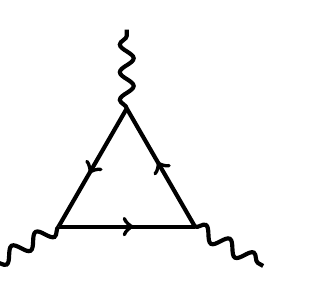
\begin{tikzpicture}[line width=1.5 pt]
	% \draw[fermion] (-30:1) -- (90:1) -- (210:1) -- cycle;
	\draw[fermion] (-30:1) -- (90:1);
	\draw[fermion] (90:1) -- (210:1);
	\draw[fermion] (210:1) -- (-30:1);
	\draw[vector] (-30:1) -- (-30:2);
	\draw[vector] (90:1) -- (90:2);
	\draw[vector] (210:1) -- (210:2);
 \end{tikzpicture}
% 
\hspace{3cm}
% 
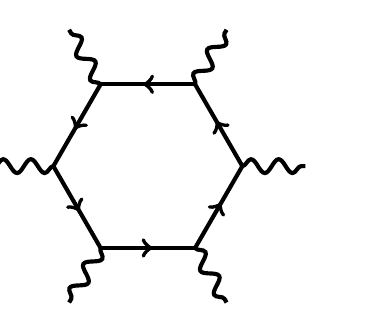
\begin{tikzpicture}[line width=1.5 pt]
	% \draw[fermion] (0:1) -- (60:1);
	% \draw[fermion] (60:1) -- (120:1);
	% \draw[fermion] (120:1) -- (180:1);
	% \draw[fermion] (180:1) -- (240:1);
	% \draw[fermion] (240:1) -- (300:1);
	% \draw[fermion] (300:1) -- (360:1);
%
	\draw[fermion] (0:1.2) -- (60:1.2);
	\draw[fermion] (60:1.2) -- (120:1.2);
	\draw[fermion] (120:1.2) -- (180:1.2);
	\draw[fermion] (180:1.2) -- (240:1.2);
	\draw[fermion] (240:1.2) -- (300:1.2);
	\draw[fermion] (300:1.2) -- (360:1.2);
%
	\draw[vector] (0:1.2) -- (0:2);
	\draw[vector] (60:1.2) -- (60:2);
	\draw[vector] (120:1.2) -- (120:2);
	\draw[vector] (180:1.2) -- (180:2);
	\draw[vector] (240:1.2) -- (240:2);
	\draw[vector] (300:1.2) -- (300:2);
 \end{tikzpicture}


\section{SUSY Cascade}
	
	
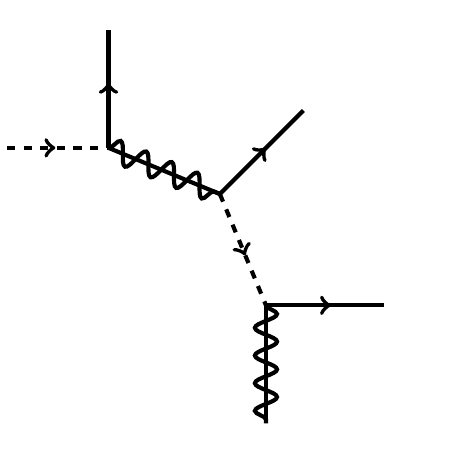
\begin{tikzpicture}[line width=1.5 pt]
	\draw[bigvector] (90:2) -- (45:2);
	\draw[fermionnoarrow] (90:2) -- (45:2);
	\draw[scalar] (45:2) -- (0:2);
	\draw[scalar] (-1.5,2) -- (0,2);
	\draw[bigvector] (2,0) -- (2,-1.5);
	\draw[fermionnoarrow] (2,0) -- (2,-1.5);
	%
	\draw[fermion] (90:2) -- (90:3.5);
	\draw[fermion] (45:2) -- (45:3.5);
	\draw[fermion] (0:2) -- (0:3.5);
\end{tikzpicture}


\section{Hadronic interactions}

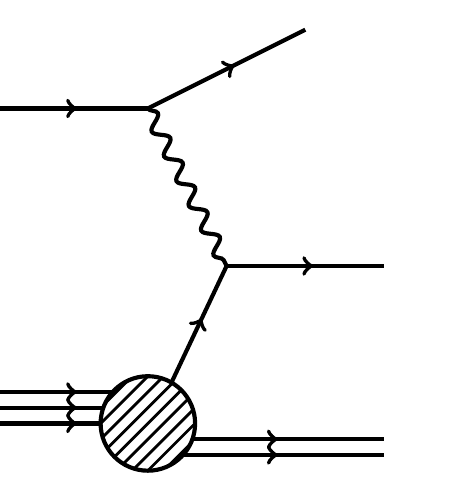
\begin{tikzpicture}[line width=1.5 pt, scale=2]
	% \draw[fermion](145:1) -- (145:.3cm);
	% 	\node at (145:1.15) {$\chi$};
	% \draw[fermion](215:1) -- (215:.3cm);
	% 	\node at (215:1.2) {SM};
	% \draw[fermionbar](35:1) -- (35:.3cm);
	% 	\node at (35:1.15) {$\chi$};
	% \draw[fermionbar](-35:1) -- (-35:.3cm);
	% 	\node at (-35:1.2) {SM};
	% \draw[fill=black] (0,0) circle (.3cm);
	% \draw[fill=white] (0,0) circle (.29cm);
	\draw[fermion] (-1,2) -- (0,2);
	\draw[fermion] (0,2) -- (1,2.5);
	\draw[vector] (0,2) -- (.5,1);
	% \draw[fermion] (0,0) -- (.5,1);
	\draw[fermion] (.5,1) -- (1.5,1);
	\draw[fermion] (60:.3) -- (.5,1);
	%
	\draw[fermion] (-1,.2) -- (0,.2);
	\draw[fermion] (-1,.1) -- (0,.1);
	\draw[fermion] (-1,0) -- (0,0);
	%
	\draw[fermion] (0,-.1) -- (1.5,-0.1);
	\draw[fermion] (0,-.2) -- (1.5,-0.2);
	\fill[white] (0,0) circle (.3);
	\begin{scope}
    	\clip (0,0) circle (.3cm);
    	\foreach \x in {-.9,-.8,...,.3}
			\draw[line width=1 pt] (\x,-.3) -- (\x+.6,.3);
  	\end{scope}
	\draw[fermionnoarrow] (0,0) circle (.3);
 \end{tikzpicture}

\vspace{1cm}

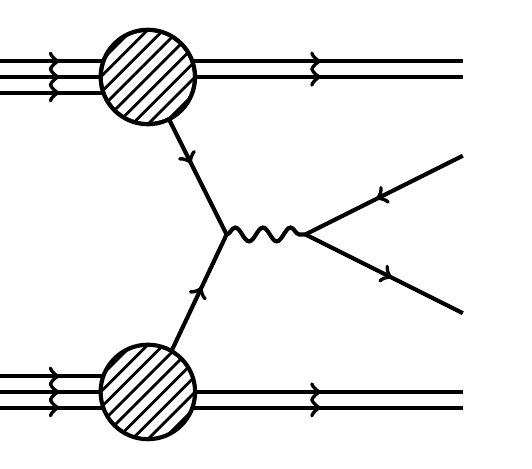
\begin{tikzpicture}[line width=1.5 pt, scale=2]
	\draw[fermion] (-1,2.1) -- (-.2,2.1);
	\draw[fermion] (-1,2) -- (-.2,2);
	\draw[fermion] (-1,1.9) -- (-.2,1.9);
	%
	\draw[fermion] (0,2) -- (2,2);
	\draw[fermion] (0,2.1) -- (2,2.1);
	\draw[fermion] (0,2) -- (.5,1);
	% \draw[fermion] (0,0) -- (.5,1);
	\draw[vector] (.5,1) -- (1,1);
	\draw[fermion] (2,1.5) -- (1,1);
	\draw[fermion] (1,1) -- (2,.5);
	%
	\draw[fermion] (60:.3) -- (.5,1);
	%
	\draw[fermion] (-1,.1) -- (-.2,.1);
	\draw[fermion] (-1,0) -- (-.2,0);
	\draw[fermion] (-1,-.1) -- (-.2,-.1);
	%
	\draw[fermion] (0,0) -- (2,0);
	\draw[fermion] (0,-.1) -- (2,-.1);
	\fill[white] (0,0) circle (.3);
%
	\begin{scope}
    	\clip (0,0) circle (.3cm);
    	\foreach \x in {-.9,-.8,...,.3}
			\draw[line width=1 pt] (\x,-.3) -- (\x+.6,.3);
  	\end{scope}
	\draw[fermionnoarrow] (0,0) circle (.3);
%	
	\begin{scope}[shift={(0,2)}]
		\fill[white] (0,0) circle (.3);
    	\clip (0,0) circle (.3cm);
    	\foreach \x in {-.9,-.8,...,.3}
			\draw[line width=1 pt] (\x,-.3) -- (\x+.6,.3);
		\draw[fermionnoarrow] (0,0) circle (.3);
  	\end{scope}
	\draw[fermionnoarrow] (0,2) circle (.3);
 \end{tikzpicture}



\section{Flavor (box and penguins)}
	
	
	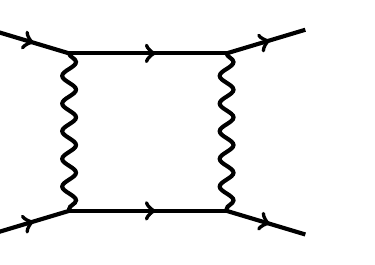
\begin{tikzpicture}[line width=1.5 pt, scale=1]
		\draw[fermion] (-1,2.3) -- (0,2);
		\draw[fermion] (0,2) -- (2,2);
		\draw[fermion] (2,2) -- (3,2.3);
		% 
		\draw[fermion] (-1,-.3) -- (0,0);
		\draw[fermion] (0,0) -- (2,0);
		\draw[fermion] (2,0) -- (3,-.3);
		%
		\draw[vector] (0,2) -- (0,0);
		\draw[vector] (2,2) -- (2,0);
	\end{tikzpicture}
	%
	%
	\hspace{3cm}
	%
	%
	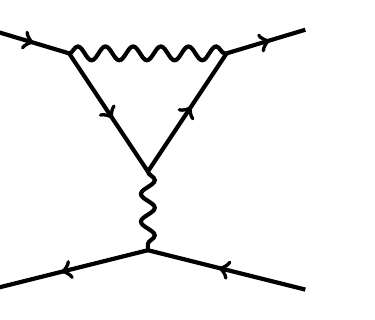
\begin{tikzpicture}[line width=1.5 pt, scale=1]
		\draw[fermion] (-1,2.3) -- (0,2);
		\draw[vector] (0,2) -- (2,2);
		\draw[fermion] (2,2) -- (3,2.3);
		%
		\draw[fermion] (0,2) -- (1,.5); 
		\draw[fermion] (1,.5) -- (2,2);
		%
		\draw[vector] (1,.5) -- (1,-.5);
		\draw[fermion] (3,-1) -- (1,-.5);
		\draw[fermion] (1,-.5) -- (-1,-1);
	\end{tikzpicture}
	
	
\section{Multiloop}


		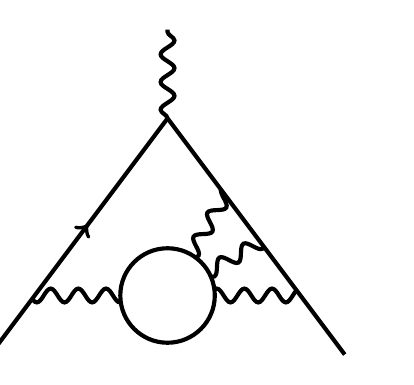
\begin{tikzpicture}[line width=1.5 pt, scale=1.5]
			\begin{scope}
				\clip (-1.5,-.5) -- (0,1.5) -- (1.5, -.5) -- cycle;
				\draw[vector] (-2,0) -- (2,0);
				\draw[vector] (0,0) -- (30:2);
				\draw[vector] (0,0) -- (60:2);
			\end{scope}
			\fill[white] (0,0) circle (.4);
			\begin{scope}
						% 	    	\clip (0,0) circle (.4cm);
						% 		    	\foreach \x in {-.9,-.8,...,.3}
						% \draw[line width=1 pt] (\x,-.3) -- (\x+.6,.3);
		  	\end{scope}
			\draw[fermionnoarrow] (0,0) circle (.4);
			% \draw[fermion] (-.4,0) arc (180:90:.4);
			% \begin{scope}[shift={(0,2)}]
			% 	\fill[white] (0,0) circle (.3);
			% 		    	\clip (0,0) circle (.3cm);
			% 		    	\foreach \x in {-.9,-.8,...,.3}
			% 		\draw[line width=1 pt] (\x,-.3) -- (\x+.6,.3);
			% 	\draw[fermionnoarrow] (0,0) circle (.3);
			% 		  	\end{scope}
			\draw[fermion] (-1.5,-.5) -- (0,1.5);
			\draw[fermionnoarrow] (0,1.5) -- (1.5,-.5);
			% \draw[fermion] (0,1.5) -- (60:2);
			% \draw[fermionnoarrow] (60:2) -- (1.5,-.5);
			\draw[vector] (0,1.5) -- (0,2.25);
		\end{tikzpicture}


\section{Renormalization}

\vspace{1em}
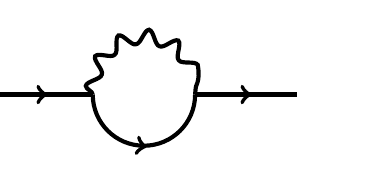
\begin{tikzpicture}[line width=1.5 pt, scale=1.3]
	\draw[fermionbar] (0:1)--(0,0);
	% \node at (-140:1.2) {$e$};
	% \node at (140:1.2) {$e$};
	% \node at (.5,.3) {$\gamma$};	
	\draw[vector] (1,0) arc (180:0:.5);
	\draw[fermionbar] (2,0) arc (0:-180:.5);
	\draw[fermion] (2,0) --(3,0);
	% \node at (2.5,.3) {$\gamma$};	
\end{tikzpicture}

\vspace{1em}
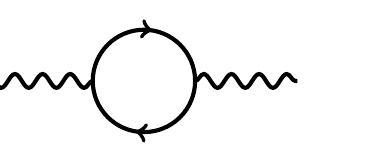
\begin{tikzpicture}[line width=1.5 pt, scale=1.3]
	\draw[vector] (0:1)--(0,0);
	\draw[fermion] (1,0) arc (180:0:.5);
	\draw[fermion] (2,0) arc (0:-180:.5);
	\draw[vector] (2,0) --(3,0);
\end{tikzpicture}


\section{Cross section}

\begin{center}
	\vspace{1em}
	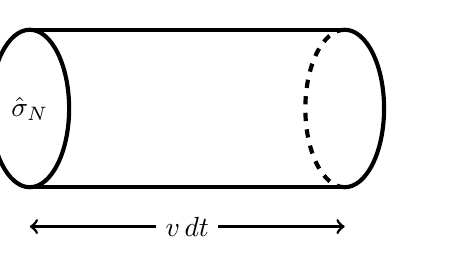
\begin{tikzpicture}[line width=1.5 pt, scale=1]
		\draw (0, 0) ellipse (.5 and 1);
		\begin{scope}[shift={(4,-1)}]
			\draw (0, 0) arc (-90:90:.5 and 1);
			\draw[scalarnoarrow] (0, 2) arc (90:270:.5 and 1);	
		\end{scope}
		\draw (0,1) -- (4,1);
		\draw (0,-1) -- (4,-1);
		\draw[line width=1 pt, <->] (0,-1.5) -- (4,-1.5);
		\node[fill=white] at (2,-1.5) {$v \, dt$};
		\node at (0,0) {$\hat\sigma_N$};
	 \end{tikzpicture}
	\vspace{1em}
\end{center}



\section{$Z$ boson}

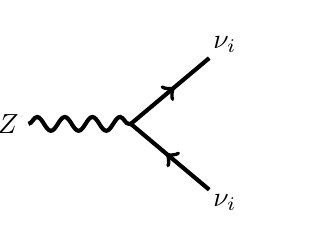
\begin{tikzpicture}[line width=1.5 pt, scale=1.3]
	\draw[fermion] (-40:1)--(0,0);
	\draw[fermionbar] (40:1)--(0,0);
	\draw[vector] (180:1)--(0,0);
	\node at (-40:1.2) {$\nu_i$};
	\node at (40:1.2) {$\nu_i$};
	\node at (180:1.2) {$Z$};	
	% \begin{scope}[shift={(3.5,0)}]
	% 	\draw[fermion] (-40:1)--(0,0);
	% 	\draw[fermionbar] (40:1)--(0,0);
	% 	\draw[vector] (180:1)--(0,0);
	% 	\node at (-40:1.2) {$\nu_i$};
	% 	\node at (40:1.2) {$\ell$};
	% 	\node at (180:1.4) {$W^\pm$};		
	% \end{scope}
\end{tikzpicture}
\vspace{1em}

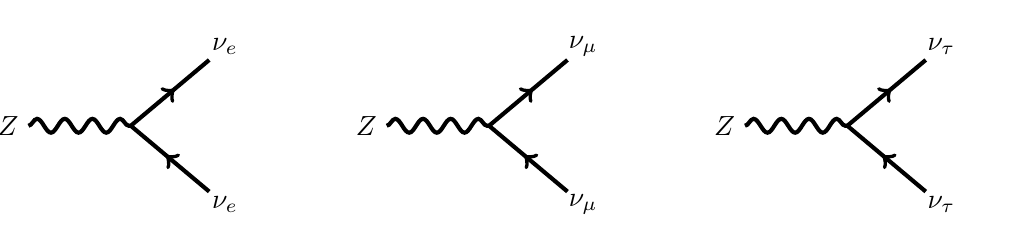
\begin{tikzpicture}[line width=1.5 pt, scale=1.3]
	\draw[fermion] (-40:1)--(0,0);
	\draw[fermionbar] (40:1)--(0,0);
	\draw[vector] (180:1)--(0,0);
	\node at (-40:1.2) {$\nu_e$};
	\node at (40:1.2) {$\nu_e$};
	\node at (180:1.2) {$Z$};	
\begin{scope}[shift={(3.5,0)}]
	\draw[fermion] (-40:1)--(0,0);
	\draw[fermionbar] (40:1)--(0,0);
	\draw[vector] (180:1)--(0,0);
	\node at (-40:1.2) {$\nu_\mu$};
	\node at (40:1.2) {$\nu_\mu$};
	\node at (180:1.2) {$Z$};		
\end{scope}
\begin{scope}[shift={(7,0)}]
	\draw[fermion] (-40:1)--(0,0);
	\draw[fermionbar] (40:1)--(0,0);
	\draw[vector] (180:1)--(0,0);
	\node at (-40:1.2) {$\nu_\tau$};
	\node at (40:1.2) {$\nu_\tau$};
	\node at (180:1.2) {$Z$};		
\end{scope}
\end{tikzpicture}


\section{$W$ boson}

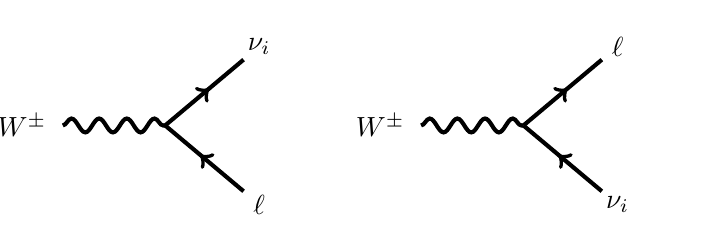
\begin{tikzpicture}[line width=1.5 pt, scale=1.3]
	\draw[fermion] (-40:1)--(0,0);
	\draw[fermionbar] (40:1)--(0,0);
	\draw[vector] (180:1)--(0,0);
	\node at (-40:1.2) {$\ell$};
	\node at (40:1.2) {$\nu_i$};
	\node at (180:1.4) {$W^\pm$};	
	\begin{scope}[shift={(3.5,0)}]
		\draw[fermion] (-40:1)--(0,0);
		\draw[fermionbar] (40:1)--(0,0);
		\draw[vector] (180:1)--(0,0);
		\node at (-40:1.2) {$\nu_i$};
		\node at (40:1.2) {$\ell$};
		\node at (180:1.4) {$W^\pm$};		
	\end{scope}
\end{tikzpicture}
\vspace{1em}


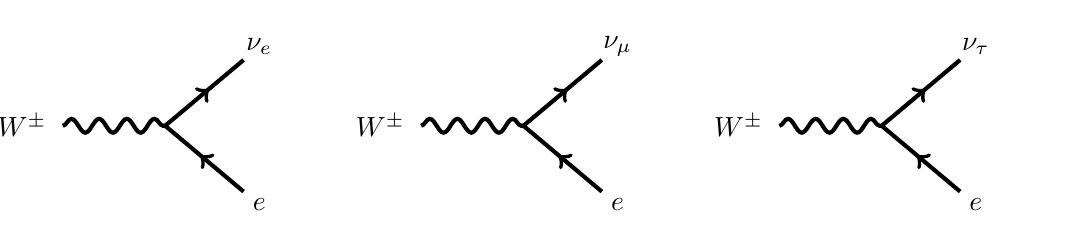
\begin{tikzpicture}[line width=1.5 pt, scale=1.3]
	\draw[fermion] (-40:1)--(0,0);
	\draw[fermionbar] (40:1)--(0,0);
	\draw[vector] (180:1)--(0,0);
	\node at (-40:1.2) {$e$};
	\node at (40:1.2) {$\nu_e$};
	\node at (180:1.4) {$W^\pm$};	
\begin{scope}[shift={(3.5,0)}]
	\draw[fermion] (-40:1)--(0,0);
	\draw[fermionbar] (40:1)--(0,0);
	\draw[vector] (180:1)--(0,0);
	\node at (-40:1.2) {$e$};
	\node at (40:1.2) {$\nu_\mu$};
	\node at (180:1.4) {$W^\pm$};		
\end{scope}
\begin{scope}[shift={(7,0)}]
	\draw[fermion] (-40:1)--(0,0);
	\draw[fermionbar] (40:1)--(0,0);
	\draw[vector] (180:1)--(0,0);
	\node at (-40:1.2) {$e$};
	\node at (40:1.2) {$\nu_\tau$};
	\node at (180:1.4) {$W^\pm$};		
\end{scope}
\end{tikzpicture}
%
\vspace{.5em}

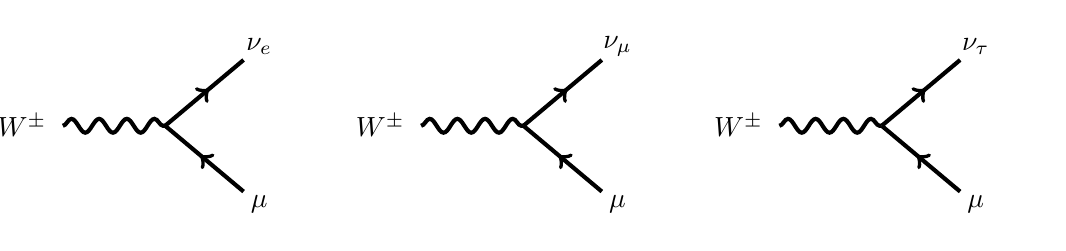
\begin{tikzpicture}[line width=1.5 pt, scale=1.3]
	\draw[fermion] (-40:1)--(0,0);
	\draw[fermionbar] (40:1)--(0,0);
	\draw[vector] (180:1)--(0,0);
	\node at (-40:1.2) {$\mu$};
	\node at (40:1.2) {$\nu_e$};
	\node at (180:1.4) {$W^\pm$};	
\begin{scope}[shift={(3.5,0)}]
	\draw[fermion] (-40:1)--(0,0);
	\draw[fermionbar] (40:1)--(0,0);
	\draw[vector] (180:1)--(0,0);
	\node at (-40:1.2) {$\mu$};
	\node at (40:1.2) {$\nu_\mu$};
	\node at (180:1.4) {$W^\pm$};		
\end{scope}
\begin{scope}[shift={(7,0)}]
	\draw[fermion] (-40:1)--(0,0);
	\draw[fermionbar] (40:1)--(0,0);
	\draw[vector] (180:1)--(0,0);
	\node at (-40:1.2) {$\mu$};
	\node at (40:1.2) {$\nu_\tau$};
	\node at (180:1.4) {$W^\pm$};		
\end{scope}
\end{tikzpicture}
%
\vspace{.5em}

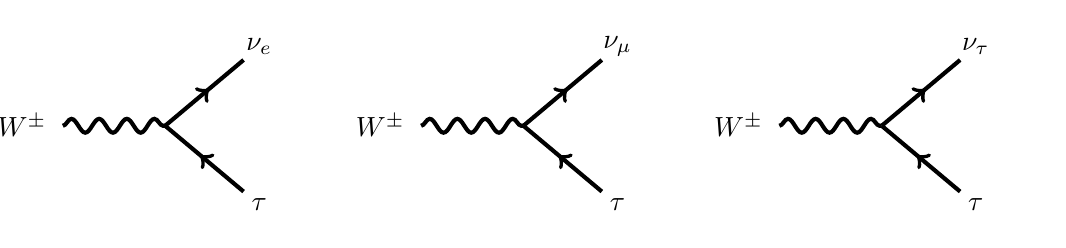
\begin{tikzpicture}[line width=1.5 pt, scale=1.3]
	\draw[fermion] (-40:1)--(0,0);
	\draw[fermionbar] (40:1)--(0,0);
	\draw[vector] (180:1)--(0,0);
	\node at (-40:1.2) {$\tau$};
	\node at (40:1.2) {$\nu_e$};
	\node at (180:1.4) {$W^\pm$};	
\begin{scope}[shift={(3.5,0)}]
	\draw[fermion] (-40:1)--(0,0);
	\draw[fermionbar] (40:1)--(0,0);
	\draw[vector] (180:1)--(0,0);
	\node at (-40:1.2) {$\tau$};
	\node at (40:1.2) {$\nu_\mu$};
	\node at (180:1.4) {$W^\pm$};		
\end{scope}
\begin{scope}[shift={(7,0)}]
	\draw[fermion] (-40:1)--(0,0);
	\draw[fermionbar] (40:1)--(0,0);
	\draw[vector] (180:1)--(0,0);
	\node at (-40:1.2) {$\tau$};
	\node at (40:1.2) {$\nu_\tau$};
	\node at (180:1.4) {$W^\pm$};		
\end{scope}
\end{tikzpicture}


\section{Dark Matter}


\begin{center}
	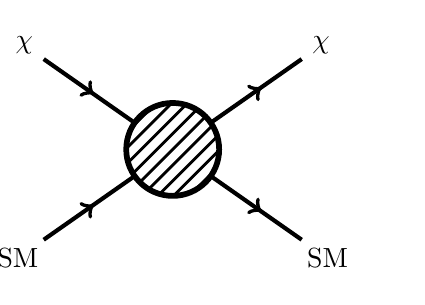
\begin{tikzpicture}[line width=1.5 pt, scale=2]
		\draw[fermion](145:1) -- (145:.3cm);
			\node at (145:1.15) {$\chi$};
		\draw[fermion](215:1) -- (215:.3cm);
			\node at (215:1.2) {SM};
		\draw[fermionbar](35:1) -- (35:.3cm);
			\node at (35:1.15) {$\chi$};
		\draw[fermionbar](-35:1) -- (-35:.3cm);
			\node at (-35:1.2) {SM};
		\draw[fill=black] (0,0) circle (.3cm);
		\draw[fill=white] (0,0) circle (.29cm);
		\begin{scope}
	    	\clip (0,0) circle (.3cm);
	    	\foreach \x in {-.9,-.8,...,.3}
				\draw[line width=1 pt] (\x,-.3) -- (\x+.6,.3);
	  	\end{scope}
	 \end{tikzpicture}	
\end{center}



\section{Coleman Weinberg}

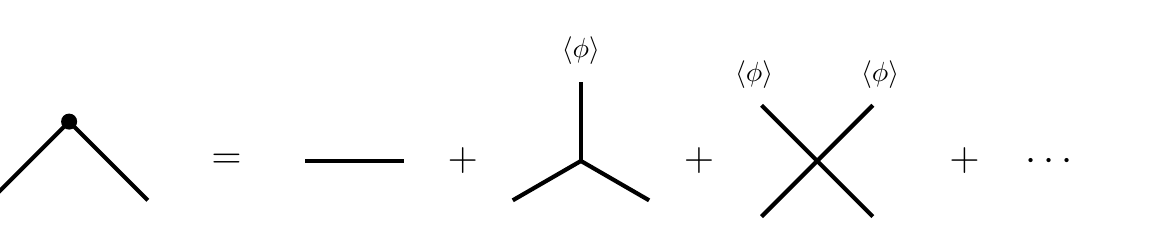
\begin{tikzpicture}[line width=1.5 pt]
	\draw (-1,-.5) -- (0,.5) -- (1,-.5);
	\draw[fill=black] (0,.5) circle (.075cm);
	\node at (2,0) {\Large=};
	\draw (3,0) -- (4.25,0);
	\node at (5,0) {\Large+};
	\draw (-30:1)+(6.5,0) -- (6.5,0);
	\draw (90:1)+(6.5,0) -- (6.5,0);
	\draw (210:1)+(6.5,0) -- (6.5,0);
	\node at (6.5,1.4) {$\langle \phi\rangle$};
	\node at (8,0) {\Large+};
	\draw (45:1)+(9.5,0) -- (9.5,0);
	\draw (135:1)+(9.5,0) -- (9.5,0);
	\draw (225:1)+(9.5,0) -- (9.5,0);
	\draw (315:1)+(9.5,0) -- (9.5,0);
	\node at (8.7,1.1) {$\langle \phi\rangle$};
	\node at (10.3,1.1) {$\langle \phi\rangle$};
	\node at (12,0) {\Large$+\hspace{.5cm}\cdots$};
 \end{tikzpicture}





\section*{Acknowledgements}

...
%
%
This work is supported in part by the NSF grant number PHY-0355005, an NSF graduate research fellowship, and a Paul \& Daisy Soros Fellowship For New Americans. The contents of this article do not necessarily represent the views of either institution.




















\appendix

% \section{Miscellaneous}
% \label{app:misc}
% 
% 
% \subsection{Direct detection recoil}
% 
% \begin{center}
% 	\begin{tikzpicture}[line width=1 pt, scale=1.5]
% 		\draw[<->, line width=1.5 pt] (0,2.5) -- (0,0) -- (4,0);
% 		\draw (0,0) rectangle (3,.5);
% 		\begin{scope}
% 	    	\clip (0,0) rectangle (3,.5);
% 	    	\foreach \x in {-1.9,-1.8,...,3.3}
% 				\draw[line width=.2 pt] (\x,-.3) -- (\x+1.2,.6);
% 	  	\end{scope}
% 		% \draw (0,.5) rectangle (2.2,1);
% 		% \draw (0,1) rectangle (1.3,1.5);
% 		% \draw (0,1.5) rectangle (.5,2);
% 		\node at (-.4, 2.5) {$\displaystyle \frac{dR}{dE_R}$};
% 		\node at (4, -.3) {$\displaystyle E_R$};
% 		\draw (3,.05) -- (3,-.1);
% 		\node at (3, -.3) {$\displaystyle E_ir$};
% 	 \end{tikzpicture}
% 	\quad\quad\quad\quad
% 	\begin{tikzpicture}[line width=1 pt, scale=1.5]
% 		\draw[<->, line width=1.5 pt] (0,2.5) -- (0,0) -- (4,0);
% 		\draw (0,0) rectangle (3,.5);
% 		\begin{scope}
% 	    	\clip (0,0) rectangle (3,.5);
% 	    	\foreach \x in {-1.9,-1.8,...,3.3}
% 				\draw[line width=.2 pt] (\x,-.3) -- (\x+1.2,.6);
% 	  	\end{scope}
% 		\draw (0,.5) rectangle (2.0,1);
% 		\draw (0,1) rectangle (1.0,1.5);
% 		\draw (0,1.5) rectangle (.5,2);
% 		\node at (-.4, 2.5) {$\displaystyle \frac{dR}{dE_R}$};
% 		\node at (4, -.3) {$\displaystyle E_R$};
% 		% \draw (3,.05) -- (3,-.1);
% 		% \node at (3, -.3) {$\displaystyle E_ir$};
% 	 \end{tikzpicture}	
% \end{center}
% 
% 
% \section{Appendix}
% \label{app:}






%%%%%%%%%
% BIBLIOGRAPHY: Option 1, inline
% But I prefer using BibTex

% \begin{thebibliography}{99}
% %
% %
% %\cite{Barbieri:2000gf}
% % \bibitem{Barbieri:2000gf}
% %   R.~Barbieri and A.~Strumia,
% %  % ``The 'LEP paradox',''
% %   [arXiv:hep-ph/0007265].
% %   %%CITATION = HEP-PH/0007265;%%
% %
%
% \end{thebibliography}
% \bibliographystyle{h-physrev}


%%%%%%%%%
% BIBLIOGRAPHY: Option 2, BibTex


% \bibliographystyle{utphys.bst}
% \bibliography{Type in the name of the .bib file here, without the extension}


\end{document}

